\begin{section}{N-Body Simulations and Power Spectra}
  \label{sec:simulation}
  We use the \textsc{CUBEP$^3$M} code \cite{bib:Harnois2013} to run
  136 simulations with a box size of 300 Mpc/h and $512^3$ particles.
  The initial conditions are computed using the transfer function
  given by CAMB \cite{bib:Lewis2000} and then propagating the power
  back to $z=100$ with a linear growth factor.  The Zel'dovich
  approximation is used to calculate the displacement and velocity
  fields of the particles.  For these simulations, we use cosmological
  parameters $\Omega_M=0.321$, $\Omega_{\Lambda}=1.0-\Omega_m$,
  $h=0.67$, $\sigma_8=0.83$, and $n_s=0.96$.  Different random seeds
  are used to produce the initial conditions for different simulations
  so that they are independent of each other.

  \begin{figure}[h]
    \centering
    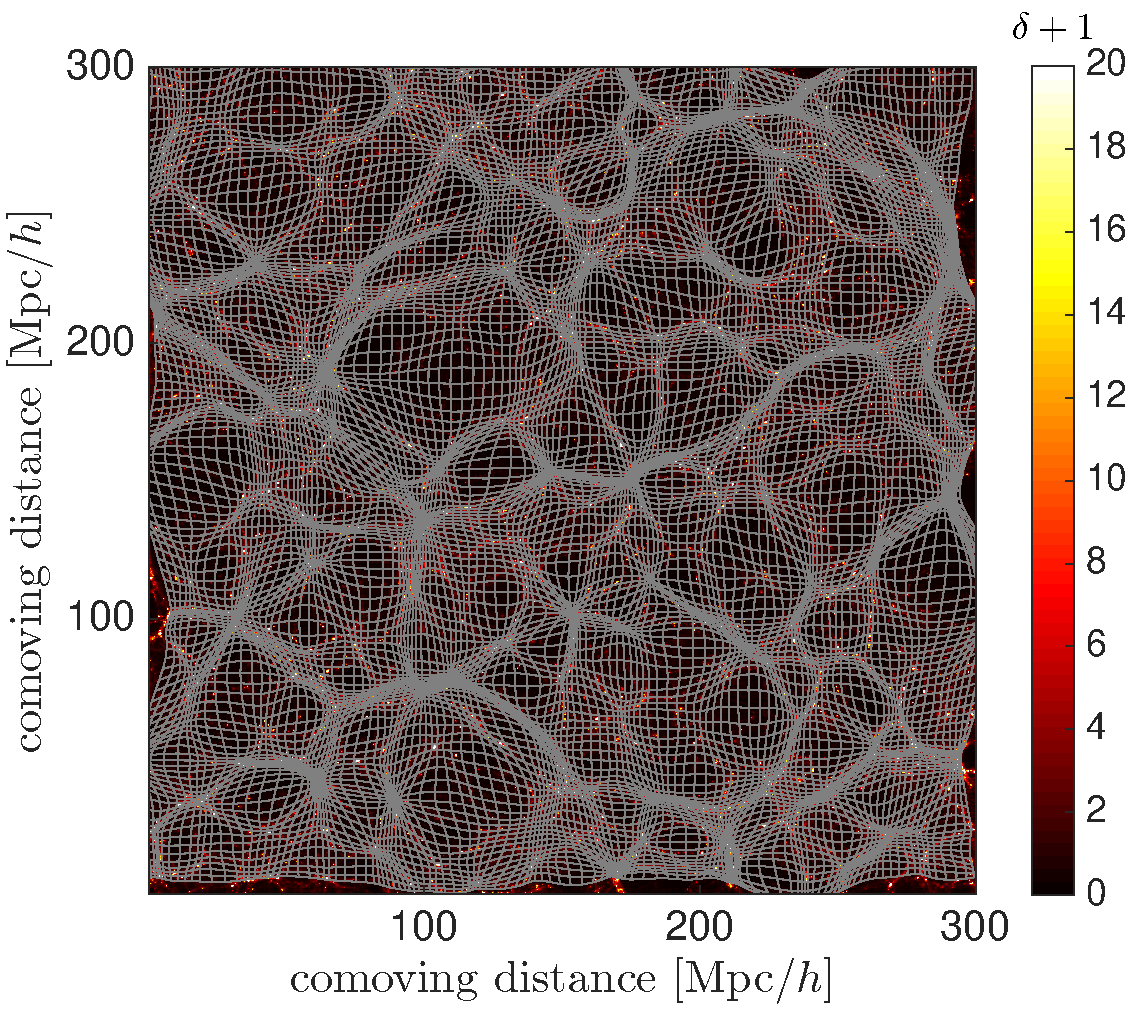
\includegraphics[width=0.45\textwidth]{fig1.pdf}
    \caption{ The 2-D projection of the deformed grid of a sample
      $N$-body simulations is shown as curved white lines.  The
      density fluctuation, $\delta\rho/\bar{\rho}$, is shown
      underneath.}
    \label{fig:simandrec}
 \end{figure}

  We use Cloud-In-Cell (CIC) interpolation to estimate the density
  contrast $\delta_S=\delta\rho/\rho-1$ from the particles.  We then
  apply the MM reconstruction to these fields with a resolution of
  $128^3$ cells.  A 2D projection of the deformed grids and the
  original density field are given in Fig. \ref{fig:simandrec}.  As
  expected, there is no grid crossing after reconstruction.
 
 The cross power spectrum, $P_{ij}(k)$, is defined as
 \begin{align}
   \langle \delta_i(\bm{k})\delta_j(\bm{k'}) \rangle =
   (2\pi)^3 P_{ij}(k) \delta_D(\bm{k}-\bm{k'}),
 \end{align}
 where $\delta_{i}$ and $\delta_j$ are density contrasts and
 $\delta_D$ is the Dirac delta funciton. We typically consider instead
 the dimensionless power spectrum, $\Delta_{ij}^2(k)$, defined as
 \begin{align}
   \Delta_{ij}^2(k) \equiv \frac{k^3 P_{ij}(k)}{2\pi ^2}.
 \end{align}
 In the left panel of Fig.~\ref{fig:cp}, we show the matter auto power
 spectrum ($i=j$) of linear theory density fields ($\delta_L$), from
 the simulation results ($\delta_S$) and after reconstruction
 ($\delta_R=-\nabla^2\phi$).  For the simulation and reconstruction
 results, we use the average value of all 136 simulations and show
 $1\sigma$ variances as error bars.  To determine the correlation
 between fields, we compute the cross correlation coefficient
 $r_{ij}(k) = P_{ij}/\sqrt{P_{ii}P_{jj}}$.  In the right panel of
 Fig.~\ref{fig:cp}, we show $r_{SL}$ and $r_{RL}$.  We see that the
 reconstructed field is much more highly correlated with the linear
 field than the simulation field is.  Specifically, we find that the
 scale at which $r(k)=1/2$ drops from $k\simeq 0.2$ h/Mpc to
 $0.6$ h/Mpc.  In comparison with the results of \citet{bib:ZhuH2016},
 we find the correlation coefficient falls off at slightly lower
 wavenumbers which we attribute to using lower resolution simulations.

  \begin{figure*}
    \centering
    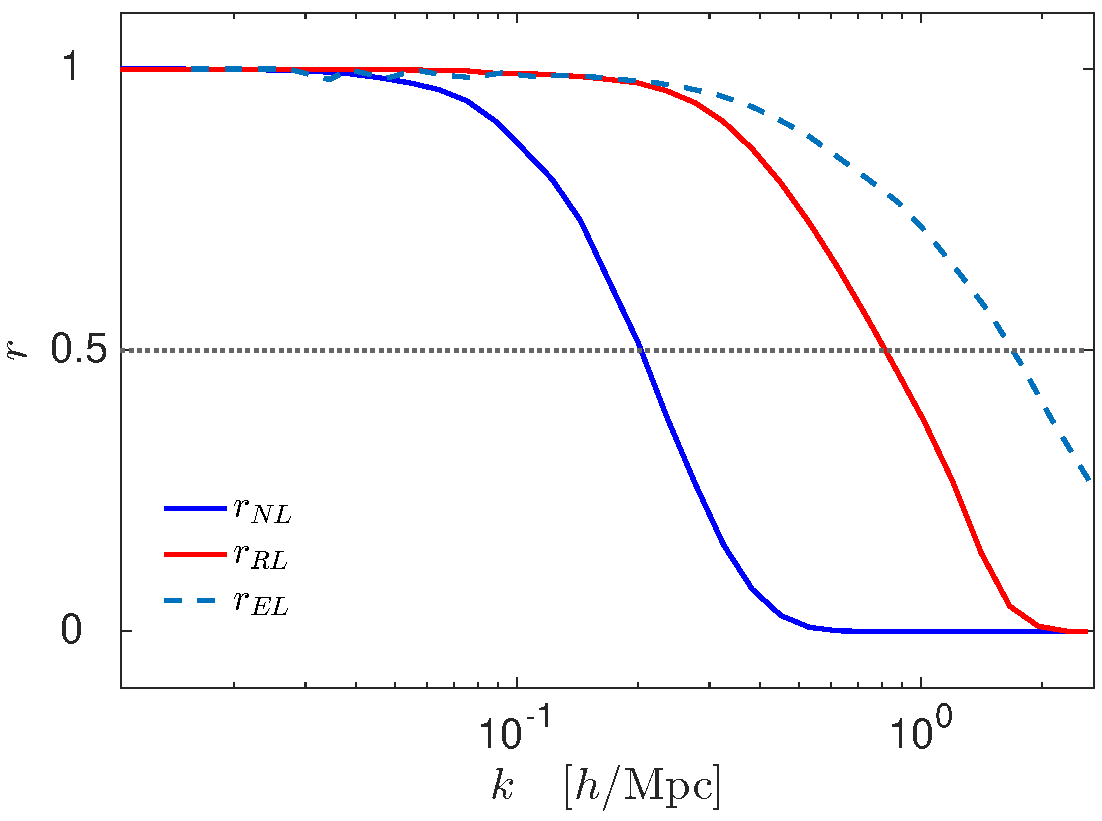
\includegraphics[width=0.48\textwidth]{fig2b.pdf}
    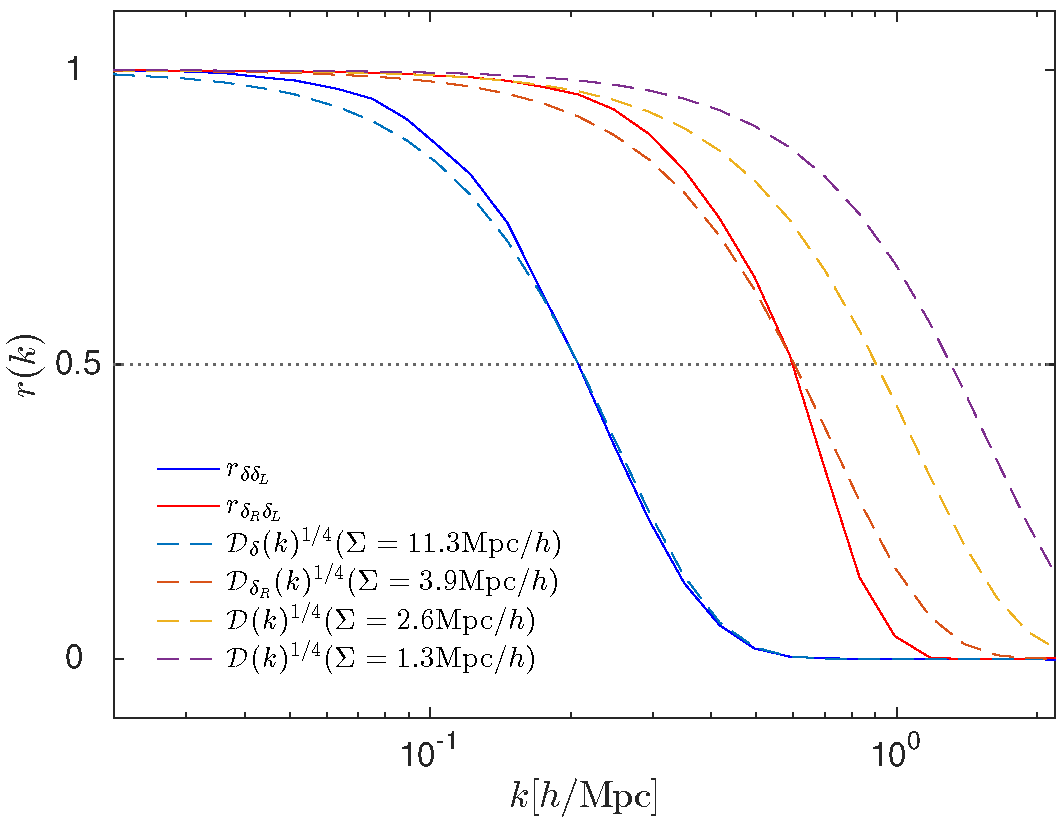
\includegraphics[width=0.455\textwidth]{fig2a.pdf}
    \caption{{\it Left.} The dimensionless power spectrum computed via
      linear theory (black), the mean value of 136 $N$-body
      simulations with $1\sigma$ error bars (blue), and reconstruction
      of the simulations (red).  {\it Right.} The cross correlation
      function (solid lines) $r_{SL}$ (blue) and
      $r_{RL}$ (red), and BAO damping models (dash
      lines).}
    \label{fig:cp}
  \end{figure*}


\end{section}

